%=================================================================
% CSE 4345 — Big Data Analytics
% Week 2, Part 1: Challenges of Big Data — Extraction, Integration
%                 and Heterogeneous Information
% Department of CSE, Premier University
%
% Part 1 covers: Introduction (silo problem) · Types of Heterogeneity
%               · ETL and ELT Paradigms · Data Quality & Provenance
%               · Ivy League Alignment · Student Assessment
% Part 2 covers: Halevy et al. (2006) · HL7/FHIR Case Study
%=================================================================

\documentclass[aspectratio=169,10pt]{beamer}

%---------- Packages ----------
\usepackage[utf8]{inputenc}
\usepackage[T1]{fontenc}
\usepackage{booktabs}
\usepackage{xcolor}
\usepackage{tikz}
\usetikzlibrary{shapes.geometric, positioning, arrows.meta,
                decorations.pathreplacing, calc}
\usepackage{amsmath}
\usepackage{graphicx}
\usepackage{multicol}
\usepackage{enumerate}
\usepackage{array}

%---------- Theme ----------
\usetheme{Madrid}

%---------- Premier University Color Identity ----------
\definecolor{PUNavy}{RGB}{10,36,99}
\definecolor{PUGold}{RGB}{197,151,37}
\definecolor{PULightBlue}{RGB}{210,228,255}
\definecolor{PUTeal}{RGB}{0,100,100}
\definecolor{PUGray}{RGB}{90,90,90}
\definecolor{PURed}{RGB}{160,30,30}
\definecolor{PUGreen}{RGB}{30,120,60}
\definecolor{PUOrange}{RGB}{200,100,20}

\setbeamercolor{palette primary}{bg=PUNavy, fg=white}
\setbeamercolor{palette secondary}{bg=PUNavy!85, fg=white}
\setbeamercolor{palette tertiary}{bg=PUNavy!70, fg=white}
\setbeamercolor{palette quaternary}{bg=PUNavy, fg=white}
\setbeamercolor{structure}{fg=PUNavy}
\setbeamercolor{title}{bg=PUNavy, fg=PUGold}
\setbeamercolor{subtitle}{fg=white}
\setbeamercolor{frametitle}{bg=PUNavy, fg=PUGold}
\setbeamercolor{alerted text}{fg=PUGold!85!black}
\setbeamercolor{block title}{bg=PUNavy, fg=white}
\setbeamercolor{block body}{bg=PULightBlue!45}
\setbeamercolor{block title alerted}{bg=PUGold!80!black, fg=white}
\setbeamercolor{block body alerted}{bg=PUGold!12}
\setbeamercolor{block title example}{bg=PUTeal, fg=white}
\setbeamercolor{block body example}{bg=PUTeal!10}
\setbeamercolor{section in toc}{fg=PUNavy}
\setbeamercolor{itemize item}{fg=PUGold!80!black}
\setbeamercolor{itemize subitem}{fg=PUNavy!70}

\setbeamertemplate{navigation symbols}{}
\setbeamertemplate{itemize item}{\scriptsize\raise1.5pt\hbox{\textbullet}}
\setbeamertemplate{itemize subitem}{\scriptsize\raise1pt\hbox{--}}

%---------- Section separator ----------
\AtBeginSection[]{
  \begin{frame}[plain]
    \vfill
    \centering
    \begin{beamercolorbox}[sep=12pt,center,shadow=true,rounded=true]{block title}
      \usebeamerfont{title}\insertsectionhead\par
    \end{beamercolorbox}
    \vfill
  \end{frame}
}

%---------- Title metadata ----------
\title[CSE 4345 \textbar{} Week 2, Part 1]{CSE 4345: Big Data Analytics}
\subtitle{Week 2, Part 1 \textemdash\ Challenges of Big Data: Extraction,
          Integration \& Heterogeneous Information}
\author[Dept.\ of CSE]{Department of Computer Science \& Engineering\\[4pt]
       \small Premier University, Chittagong}
\institute{}
\date{Semester 2026}

%=================================================================
\begin{document}
%=================================================================

%----------------------------------------------------------------
% TITLE SLIDE
%----------------------------------------------------------------
\begin{frame}
  \titlepage
\end{frame}

%----------------------------------------------------------------
% COURSE INFO
%----------------------------------------------------------------
\begin{frame}{Course \& Lecture Information}
  \begin{columns}[T]
    \column{0.47\textwidth}
      \begin{block}{Lecture Identity}
        \begin{tabular}{ll}
          \textbf{Course:}    & CSE 4345 \\
          \textbf{Week / Part:} & 2 of 11 \textbar\ Part 1 of 2 \\
          \textbf{CLO:}       & CLO2 \\
          \textbf{PLO:}       & PLO(b), PLO(c) \\
        \end{tabular}
      \end{block}
      \vspace{6pt}
      \begin{alertblock}{CLO2}
        \textit{``Analyse the existing challenges in Big Data''}
      \end{alertblock}
      \vspace{6pt}
      \begin{block}{Prerequisite Recall}
        \small Week 1 established the \textbf{3Vs}\textemdash Volume, Velocity, Variety.  Week 2 dives into \textbf{Variety} in depth: what happens when you must integrate data from tens of heterogeneous sources.
      \end{block}

    \column{0.50\textwidth}
      \begin{exampleblock}{Part 1 Covers}
        \begin{itemize}
          \item The data silo problem
          \item Four types of heterogeneity
          \item ETL: Extract, Transform, Load (in depth)
          \item ELT: The data lake paradigm
          \item Data quality dimensions \& provenance
          \item Entity resolution
          \item Ivy League alignment
          \item Student assessment pool
        \end{itemize}
      \end{exampleblock}
      \vspace{4pt}
      \begin{block}{Part 2 Preview}
        Seminal paper: Halevy, Rajaraman \& Ordille (2006)\\
        Case Study: HL7/FHIR \& Healthcare Interoperability
      \end{block}
  \end{columns}
\end{frame}

%----------------------------------------------------------------
% AGENDA
%----------------------------------------------------------------
\begin{frame}{Lecture Agenda}
  \tableofcontents
\end{frame}

%================================================================
\section{The Data Silo Problem}
%================================================================

\begin{frame}{Organisations Are Data-Rich, Insight-Poor}
  \begin{columns}[T]
    \column{0.54\textwidth}
      \begin{block}{The Reality of Enterprise Data (2024)}
        A mid-sized bank in Bangladesh typically holds customer data in:
        \begin{itemize}
          \item \textbf{Core banking system} (Oracle RDBMS)
          \item \textbf{Mobile banking app} (MySQL + NoSQL)
          \item \textbf{Loan origination system} (separate legacy RDBMS)
          \item \textbf{Call centre CRM} (Salesforce cloud)
          \item \textbf{ATM transaction logs} (flat CSV files, nightly dump)
          \item \textbf{AML / fraud reports} (Excel spreadsheets)
          \item \textbf{Regulatory filings} (Bangladesh Bank XML schemas)
        \end{itemize}
      \end{block}
      \vspace{4pt}
      \begin{alertblock}{The Silo Consequence}
        A customer who complains about a loan payment appears as \textbf{seven different, unlinked records} across these systems.  No single analyst can see the full picture.
      \end{alertblock}

    \column{0.43\textwidth}
      \begin{center}
      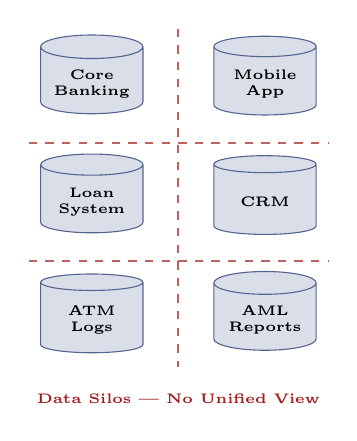
\begin{tikzpicture}[
          db/.style={cylinder, draw=PUNavy!70, fill=PUNavy!15,
                     minimum height=1.0cm, minimum width=1.3cm,
                     shape border rotate=90, aspect=0.25,
                     font=\tiny\bfseries, align=center},
          wall/.style={draw=PURed!70, dashed, thick}
        ]
        % Silos
        \node[db] (a) at (0,  2.4) {Core\\Banking};
        \node[db] (b) at (2.2,2.4) {Mobile\\App};
        \node[db] (c) at (0,  0.9) {Loan\\System};
        \node[db] (d) at (2.2,0.9) {CRM};
        \node[db] (e) at (0, -0.6) {ATM\\Logs};
        \node[db] (f) at (2.2,-0.6) {AML\\Reports};

        % Walls between them (no connections)
        \draw[wall] (1.1, 3.1) -- (1.1,-1.2);
        \draw[wall] (-0.8,1.65) -- (3.0,1.65);
        \draw[wall] (-0.8,0.15) -- (3.0,0.15);

        % Label
        \node[font=\tiny\bfseries, PURed] at (1.1,-1.6)
              {Data Silos — No Unified View};
      \end{tikzpicture}
      \end{center}
      \vspace{4pt}
      \begin{exampleblock}{A 2019 Forrester Study}
        \small \textbf{73\%} of enterprise data is never analysed.  The primary reason: \textbf{integration complexity}.
      \end{exampleblock}
  \end{columns}
\end{frame}

%----------------------------------------------------------------
\begin{frame}{The Integration Challenge at Scale}
  \begin{columns}[T]
    \column{0.52\textwidth}
      \begin{block}{The Core Problem Statement}
        \textit{``Given a set of heterogeneous, autonomous data sources, provide the user with a \textbf{unified, transparent query interface} that gives a single coherent view of all data.''}\\
        \hfill\textemdash\,Halevy, Rajaraman \& Ordille (2006)
      \end{block}
      \vspace{6pt}
      \textbf{Three fundamental dimensions of difficulty:}
      \begin{enumerate}
        \item \textbf{Heterogeneity}: Sources use different schemas, formats, vocabularies, and update cadences
        \item \textbf{Autonomy}: Each source is independently managed; the integration layer cannot change the source
        \item \textbf{Scale}: The volume and velocity of data make manual reconciliation impossible
      \end{enumerate}

    \column{0.45\textwidth}
      \renewcommand{\arraystretch}{1.3}
      \begin{tabular}{p{2.2cm}p{3.8cm}}
        \toprule
        \textbf{Challenge} & \textbf{Big Data Dimension} \\
        \midrule
        Heterogeneity & Variety \textemdash\ different formats, schemas \\
        Scale & Volume \textemdash\ 100 TB cannot be loaded into memory \\
        Noise \& gaps & Veracity \textemdash\ sensor dropout, OCR errors \\
        Provenance & Regulatory \textemdash\ GDPR, PDPA \\
        Latency & Velocity \textemdash\ real-time vs.\ nightly batch \\
        \bottomrule
      \end{tabular}
      \vspace{6pt}
      \begin{alertblock}{Key Insight}
        The 3Vs from Week 1 were symptoms.  The integration challenge is the \textbf{engineering consequence} of those symptoms manifesting simultaneously.
      \end{alertblock}
  \end{columns}
\end{frame}

%================================================================
\section{Types of Data Heterogeneity}
%================================================================

\begin{frame}{Four Dimensions of Heterogeneity}
  \begin{center}
  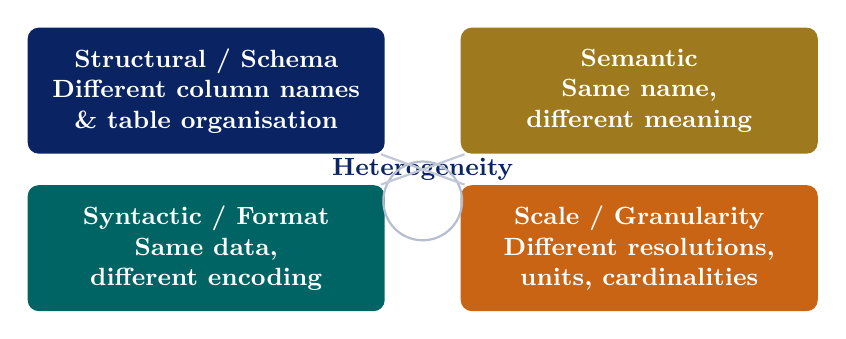
\begin{tikzpicture}[
      quad/.style={rectangle, rounded corners=4pt, minimum width=4.5cm,
                   minimum height=1.6cm, text width=4.3cm,
                   align=center, font=\small\bfseries},
      sub/.style={font=\scriptsize\normalfont}
    ]
    \node[quad, fill=PUNavy,        text=white] (A) at (0,   1.7)
          {Structural / Schema\\\sub{Different column names\\\& table organisation}};
    \node[quad, fill=PUGold!80!black, text=white] (B) at (5.5, 1.7)
          {Semantic\\\sub{Same name,\\ different meaning}};
    \node[quad, fill=PUTeal,         text=white] (C) at (0,  -0.3)
          {Syntactic / Format\\\sub{Same data,\\ different encoding}};
    \node[quad, fill=PUOrange,        text=white] (D) at (5.5,-0.3)
          {Scale / Granularity\\\sub{Different resolutions,\\ units, cardinalities}};

    % Central label
    \node[font=\bfseries\small, PUNavy] at (2.75, 0.7) {Heterogeneity};
    \draw[PUNavy!30, thick] (2.75,0.3) circle (0.5cm);

    % Lines to centre
    \foreach \n in {A,B,C,D}{
      \draw[PUNavy!25, thick] (\n) -- (2.75,0.7);
    }
  \end{tikzpicture}
  \end{center}
  \vspace{6pt}
  \begin{alertblock}{Why All Four Matter Simultaneously}
    A single integration pipeline must handle all four dimensions at once.  Solving only structural heterogeneity (schema matching) while ignoring semantic heterogeneity (meaning) produces a technically unified but analytically \textbf{misleading} dataset.
  \end{alertblock}
\end{frame}

%----------------------------------------------------------------
\begin{frame}{Structural (Schema) Heterogeneity}
  \begin{columns}[T]
    \column{0.50\textwidth}
      \begin{block}{Definition}
        Two data sources represent the \textbf{same real-world concept} using \textbf{different table structures, column names, or normalisation levels}.
      \end{block}
      \vspace{6pt}
      \textbf{Two sub-types:}
      \begin{itemize}
        \item \textbf{Naming conflicts}: Different names for the same attribute
        \begin{itemize}
          \small
          \item Source A: \texttt{cust\_id} $\leftrightarrow$ Source B: \texttt{customer\_number}
          \item Source A: \texttt{dob} $\leftrightarrow$ Source B: \texttt{birth\_date}
        \end{itemize}
        \item \textbf{Structural conflicts}: Flat vs.\ normalised schemas
        \begin{itemize}
          \small
          \item Source A: one \texttt{address} column (full address as a string)
          \item Source B: four columns (\texttt{street}, \texttt{city}, \texttt{district}, \texttt{postcode})
        \end{itemize}
      \end{itemize}
      \vspace{4pt}
      \begin{exampleblock}{Solution: Schema Mapping}
        Define transformation rules: \texttt{cust\_id} $\to$ \texttt{customer\_number}, concatenate \texttt{street + city + district} $\to$ \texttt{address}.
      \end{exampleblock}

    \column{0.47\textwidth}
      \begin{block}{Bangladesh NID Integration Example}
        \small
        \renewcommand{\arraystretch}{1.2}
        \begin{tabular}{lll}
          \toprule
          & \textbf{BREC Schema} & \textbf{MOHFW Schema} \\
          \midrule
          ID field   & \texttt{nid\_no}     & \texttt{national\_id} \\
          Full name  & \texttt{full\_name}  & \texttt{fname + lname} \\
          Birth date & \texttt{dob}         & \texttt{birth\_dt} \\
          Address    & Single string         & 5 separate columns \\
          Gender     & \texttt{M}/\texttt{F} & \texttt{1}/\texttt{2} \\
          \bottomrule
        \end{tabular}
        \vspace{4pt}
        Integrating Bangladesh Election Commission records with Ministry of Health records requires \textbf{mapping every field pair} before any query can span both.
      \end{block}
  \end{columns}
\end{frame}

%----------------------------------------------------------------
\begin{frame}{Semantic Heterogeneity}
  \begin{columns}[T]
    \column{0.50\textwidth}
      \begin{block}{Definition}
        Two data sources use the \textbf{same attribute name} (or structure) but \textbf{mean different things}, or use different vocabularies for the same concept.
      \end{block}
      \vspace{6pt}
      \textbf{Common manifestations:}
      \begin{itemize}
        \item \textbf{Homonyms}: Same word, different meaning
        \begin{itemize}
          \small
          \item \texttt{date} = admission date in Hospital A
          \item \texttt{date} = birth date in Hospital B
          \item \texttt{date} = record-entry date in Health Ministry
        \end{itemize}
        \item \textbf{Synonyms}: Different words, same concept
        \begin{itemize}
          \small
          \item \texttt{revenue} vs.\ \texttt{income} vs.\ \texttt{turnover} (same KPI, different label)
        \end{itemize}
        \item \textbf{Granularity mismatch}: ``Region'' = division in one system, district in another
        \item \textbf{Unit conflicts}: Temperature in $^\circ$C vs.\ $^\circ$F; currency in BDT vs.\ USD
      \end{itemize}

    \column{0.47\textwidth}
      \begin{alertblock}{Why Semantic Heterogeneity is Hardest}
        Structural heterogeneity can often be resolved \textbf{algorithmically} (match column names, infer types).  Semantic heterogeneity requires \textbf{domain knowledge}\textemdash a machine cannot know that \texttt{date} means birth date without reading the data dictionary.
      \end{alertblock}
      \vspace{6pt}
      \begin{exampleblock}{Real Impact: Challenger Disaster (1986)}
        NASA and Morton Thiokol engineers used the word ``acceptable'' to mean different risk levels when discussing O-ring failures.  This semantic mismatch contributed to the decision to launch.\\[4pt]
        \textit{Source: Vaughan, D. (1996). \textit{The Challenger Launch Decision}. U.\ of Chicago Press.}
      \end{exampleblock}
  \end{columns}
\end{frame}

%----------------------------------------------------------------
\begin{frame}{Syntactic \& Scale Heterogeneity}
  \begin{columns}[T]
    \column{0.50\textwidth}
      \begin{block}{Syntactic / Format Heterogeneity}
        The \textbf{same data value} is encoded in \textbf{different formats} across sources.
      \end{block}
      \vspace{4pt}
      \textbf{Examples (all representing January 15, 2024):}
      \vspace{2pt}
      \renewcommand{\arraystretch}{1.2}
      \begin{tabular}{ll}
        \toprule
        \textbf{Format} & \textbf{Value} \\
        \midrule
        ISO 8601         & \texttt{2024-01-15} \\
        US format        & \texttt{01/15/2024} \\
        Bangladesh      & \texttt{15-01-2024} \\
        Unix epoch       & \texttt{1705276800} \\
        Bengali calendar & \texttt{01 Magh 1430} \\
        \bottomrule
      \end{tabular}
      \vspace{4pt}
      \begin{exampleblock}{Beyond Dates}
        Phone numbers: \texttt{01711-123456} vs.\ \texttt{+8801711123456} vs.\ \texttt{8801711123456}\textemdash three representations of the same Bangladeshi mobile number.
      \end{exampleblock}

    \column{0.47\textwidth}
      \begin{block}{Scale / Granularity Heterogeneity}
        Sources represent the \textbf{same domain} at \textbf{different levels of detail} or resolution.
      \end{block}
      \vspace{4pt}
      \textbf{Examples:}
      \begin{itemize}
        \item \textbf{Geographic}: One source records GPS coordinates (lat/long to 6 decimal places); another records only the district name
        \item \textbf{Temporal}: Sales DB records hourly totals; ERP records daily totals; financial system records monthly summaries
        \item \textbf{Numeric precision}: Sensor A: temperature to 0.001$^\circ$C; Sensor B: rounds to nearest integer
        \item \textbf{Aggregation}: One system reports individual transactions; another stores only daily net position
      \end{itemize}
      \vspace{4pt}
      \begin{alertblock}{Aggregation is irreversible}
        You can aggregate fine-grained data up, but you \textbf{cannot disaggregate} monthly summaries into hourly records.  Always store at the finest available granularity.
      \end{alertblock}
  \end{columns}
\end{frame}

%================================================================
\section{ETL and ELT Paradigms}
%================================================================

\begin{frame}{The ETL Process: Origin and Logic}
  \begin{columns}[T]
    \column{0.52\textwidth}
      \begin{block}{What is ETL?}
        \textbf{Extract -- Transform -- Load}: the classical approach to data integration, dominant from the 1990s through the 2010s.  Data is \textbf{transformed before it reaches the warehouse}.
      \end{block}
      \vspace{6pt}
      \textbf{Why ETL was designed this way:}
      \begin{itemize}
        \item Storage was \textbf{expensive}\textemdash only clean, structured data deserved to be stored
        \item Data warehouses (Teradata, Netezza) had \textbf{rigid schemas} that required pre-conformed data
        \item Analysts knew \emph{upfront} exactly which reports they needed\textemdash the schema was designed for known queries
        \item Regulatory compliance demanded \textbf{verified, audited} data before loading
      \end{itemize}
      \vspace{4pt}
      \begin{exampleblock}{Textbook References}
        \textbf{[SA]} Ch.\,2 $\cdot$ \textbf{[TE]} Ch.\,3
      \end{exampleblock}

    \column{0.45\textwidth}
      \begin{center}
      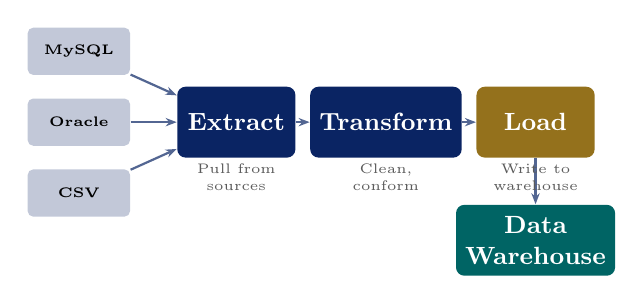
\begin{tikzpicture}[
          stage/.style={rectangle, rounded corners=3pt, fill=PUNavy,
                        text=white, minimum width=1.5cm, minimum height=0.9cm,
                        font=\small\bfseries, align=center},
          src/.style={rectangle, rounded corners=2pt, fill=PUNavy!25,
                      minimum width=1.3cm, minimum height=0.6cm,
                      font=\tiny\bfseries, align=center},
          tgt/.style={rectangle, rounded corners=3pt, fill=PUGold!75!black,
                      text=white, minimum width=1.5cm, minimum height=0.9cm,
                      font=\small\bfseries, align=center},
          arr/.style={-{Stealth[length=4pt]}, thick, PUNavy!70}
        ]
        % Sources
        \node[src] (s1) at (0, 2.0) {MySQL};
        \node[src] (s2) at (0, 1.1) {Oracle};
        \node[src] (s3) at (0, 0.2) {CSV};

        % ETL Stages
        \node[stage] (E) at (2.0, 1.1) {Extract};
        \node[stage] (T) at (3.9, 1.1) {Transform};
        \node[tgt]   (L) at (5.8, 1.1) {Load};

        % Target
        \node[tgt, fill=PUTeal, minimum width=1.6cm] (DW) at (5.8,-0.4)
              {Data\\Warehouse};

        % Arrows
        \draw[arr] (s1) -- (E);
        \draw[arr] (s2) -- (E);
        \draw[arr] (s3) -- (E);
        \draw[arr] (E)  -- (T);
        \draw[arr] (T)  -- (L);
        \draw[arr] (L)  -- (DW);

        % Labels
        \node[font=\tiny, PUGray, align=center] at (2.0, 0.4) {Pull from\\sources};
        \node[font=\tiny, PUGray, align=center] at (3.9, 0.4) {Clean,\\conform};
        \node[font=\tiny, PUGray, align=center] at (5.8, 0.4) {Write to\\warehouse};
      \end{tikzpicture}
      \end{center}
      \vspace{4pt}
      \begin{alertblock}{Key Characteristic}
        The data warehouse only ever sees \textbf{clean, structured, schema-conformed} data.  Raw data never enters.
      \end{alertblock}
  \end{columns}
\end{frame}

%----------------------------------------------------------------
\begin{frame}{ETL: The Three Phases in Depth}
  \begin{columns}[T]
    \column{0.32\textwidth}
      \begin{block}{Phase 1: Extract}
        \vspace{2pt}
        Pull data from source systems:
        \begin{itemize}
          \small
          \item \textbf{Full extract}: dump entire source table (expensive, nightly)
          \item \textbf{Incremental extract}: only changed rows since last run (CDC — Change Data Capture)
          \item \textbf{Connectors}: JDBC for RDBMS, REST APIs, SFTP for file drops
          \item Challenge: source systems may be \textbf{unavailable} during extraction window
        \end{itemize}
      \end{block}

    \column{0.32\textwidth}
      \begin{exampleblock}{Phase 2: Transform}
        \vspace{2pt}
        The most \textbf{complex} stage:
        \begin{itemize}
          \small
          \item \textbf{Cleansing}: fix nulls, remove duplicates, correct typos
          \item \textbf{Standardisation}: unify date formats, currency, units
          \item \textbf{Schema mapping}: rename columns, restructure tables
          \item \textbf{Enrichment}: join with reference tables (e.g., add district name from postcode)
          \item \textbf{Aggregation}: compute summaries (daily totals from raw transactions)
          \item \textbf{Validation}: reject rows that violate business rules
        \end{itemize}
      \end{exampleblock}

    \column{0.32\textwidth}
      \begin{alertblock}{Phase 3: Load}
        \vspace{2pt}
        Write transformed data to the target:
        \begin{itemize}
          \small
          \item \textbf{Full load}: overwrite the target table (simple, but slow)
          \item \textbf{Incremental load}: append or upsert new/changed rows
          \item \textbf{Slowly Changing Dimensions (SCD)}: preserve historical versions of records (e.g., a customer's old address)
          \item \textbf{Partitioned load}: write to date/region partitions for query performance
        \end{itemize}
      \end{alertblock}
  \end{columns}
  \vspace{8pt}
  \begin{block}{End-to-End ETL Example: Bangladeshi Garment Factory Analytics}
    \small \textbf{Extract}: Pull daily production counts from 200 factory MES systems (MySQL) + attendance records (Oracle) + fabric purchase orders (Excel SFTP drops). \textbf{Transform}: Unify factory IDs, convert shift durations to hours, handle missing values for idle machines, compute efficiency ratios. \textbf{Load}: Write to Hive-partitioned data warehouse (by factory, by week) for BGMEA compliance reporting.
  \end{block}
\end{frame}

%----------------------------------------------------------------
\begin{frame}{ELT: The Data Lake Approach}
  \begin{columns}[T]
    \column{0.52\textwidth}
      \begin{block}{What is ELT?}
        \textbf{Extract -- Load -- Transform}: Load raw data \emph{first} into a cheap, schema-flexible storage layer, then transform \emph{on demand} using Spark or Hive.
      \end{block}
      \vspace{6pt}
      \textbf{Why ELT emerged (post-2010):}
      \begin{itemize}
        \item Cloud storage costs dropped to \textbf{\$0.023/GB/month} (AWS S3)\textemdash cheap enough to store raw data
        \item \textbf{Schema-on-read} (Hive, Spark): define schema at query time, not ingest time
        \item Data scientists need \textbf{raw, unprocessed} data for ML feature engineering\textemdash ETL discards too much
        \item Transformation requirements are often \textbf{unknown} at ingest time (exploratory analytics)
        \item HDFS/S3 + Spark can transform petabytes in minutes\textemdash the ``T'' is no longer the bottleneck
      \end{itemize}

    \column{0.45\textwidth}
      \begin{center}
      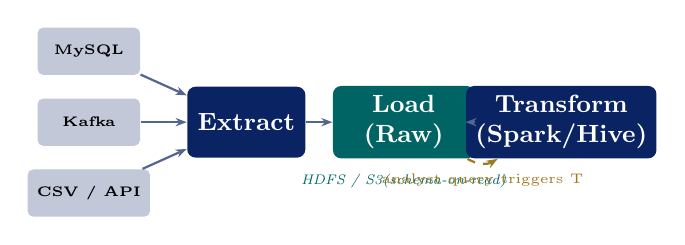
\begin{tikzpicture}[
          stage/.style={rectangle, rounded corners=3pt, fill=PUNavy,
                        text=white, minimum width=1.5cm, minimum height=0.9cm,
                        font=\small\bfseries, align=center},
          src/.style={rectangle, rounded corners=2pt, fill=PUNavy!25,
                      minimum width=1.3cm, minimum height=0.6cm,
                      font=\tiny\bfseries, align=center},
          lake/.style={rectangle, rounded corners=3pt, fill=PUTeal,
                       text=white, minimum width=1.8cm, minimum height=0.9cm,
                       font=\small\bfseries, align=center},
          arr/.style={-{Stealth[length=4pt]}, thick, PUNavy!70}
        ]
        % Sources
        \node[src] (s1) at (0, 2.0) {MySQL};
        \node[src] (s2) at (0, 1.1) {Kafka};
        \node[src] (s3) at (0, 0.2) {CSV / API};

        % ELT Stages
        \node[stage] (E)  at (2.0, 1.1) {Extract};
        \node[lake]  (DL) at (4.0, 1.1) {Load\\(Raw)};
        \node[stage] (T)  at (6.0, 1.1) {Transform\\(Spark/Hive)};

        % Arrows
        \draw[arr] (s1) -- (E);
        \draw[arr] (s2) -- (E);
        \draw[arr] (s3) -- (E);
        \draw[arr] (E)  -- (DL);
        \draw[arr] (DL) -- (T);

        % Storage label
        \node[font=\tiny\itshape, PUTeal] at (4.0, 0.35)
              {HDFS / S3\\(schema-on-read)};

        % On-demand arrow
        \draw[arr, PUGold!80!black, dashed] (DL) to[bend right=30]
              node[below, font=\tiny, PUGold!80!black]{analyst query triggers T}
              (T);
      \end{tikzpicture}
      \end{center}
      \vspace{4pt}
      \begin{alertblock}{Key Characteristic}
        Raw data \textbf{always preserved}.  Transformation is triggered \emph{by the query}, not at ingest time.  Multiple analysts can apply different transformations to the same raw data.
      \end{alertblock}
  \end{columns}
\end{frame}

%----------------------------------------------------------------
\begin{frame}{ETL vs.\ ELT: Comprehensive Comparison}
  \centering
  \renewcommand{\arraystretch}{1.45}
  \begin{tabular}{p{2.8cm}p{4.3cm}p{4.3cm}}
    \toprule
    \textbf{Dimension} & \textbf{ETL} & \textbf{ELT} \\
    \midrule
    \textbf{Transform timing} & Before loading (at ingest) & After loading (on query) \\
    \textbf{Schema} & Schema-on-write (rigid) & Schema-on-read (flexible) \\
    \textbf{Storage} & Only clean data stored & Raw \emph{and} processed data stored \\
    \textbf{Raw data} & Discarded after transform & Always preserved in data lake \\
    \textbf{Latency} & High (transform pipeline runs before data is queryable) & Low (data available immediately after load) \\
    \textbf{Best for} & Known query patterns, compliance, sensitive data & ML feature engineering, exploration, unknown future queries \\
    \textbf{Tools} & Informatica, SSIS, Talend, Ab Initio & Apache Spark + HDFS/S3, AWS Glue, dbt \\
    \textbf{Example} & Nightly bank reconciliation to Teradata DW & Netflix data lake: raw events in S3, transformed by Spark on demand \\
    \bottomrule
  \end{tabular}
  \vspace{6pt}
  \begin{alertblock}{Modern Reality: ELT Dominates for Big Data}
    The cost of storing raw data on S3/HDFS is now \emph{lower} than the cost of transforming it before load.  ELT is the de facto standard for new data lake architectures in 2024.
  \end{alertblock}
\end{frame}

%================================================================
\section{Data Quality, Provenance \& Entity Resolution}
%================================================================

\begin{frame}{Data Quality: Six Dimensions (DAMA Framework)}
  \begin{columns}[T]
    \column{0.55\textwidth}
      \renewcommand{\arraystretch}{1.4}
      \begin{tabular}{p{2.0cm}p{2.5cm}p{2.6cm}}
        \toprule
        \textbf{Dimension} & \textbf{Definition} & \textbf{Big Data Example} \\
        \midrule
        \textbf{Accuracy}    & Correctly reflects reality & GPS coordinates drifting 200 m \\
        \textbf{Completeness} & All required data present & 30\% of sensor readings missing due to network dropout \\
        \textbf{Consistency} & Data agrees across systems & Customer age is 32 in CRM but 35 in loan system \\
        \textbf{Timeliness}  & Data is current for use case & Yesterday's stock price used for real-time trade decision \\
        \textbf{Validity}    & Conforms to defined rules & Mobile number with 9 digits instead of 11 \\
        \textbf{Uniqueness}  & No duplicate records & Same customer appearing 3 times with different IDs \\
        \bottomrule
      \end{tabular}

    \column{0.42\textwidth}
      \begin{alertblock}{The ``Garbage In, Garbage Out'' Law}
        A sophisticated machine learning model trained on inaccurate, incomplete, or inconsistent data will produce \textbf{confidently wrong} predictions.  Data quality validation must happen \textbf{before} any analytics.
      \end{alertblock}
      \vspace{6pt}
      \begin{exampleblock}{Cost of Poor Quality}
        \small IBM (2016) estimated that poor data quality costs the US economy \textbf{\$3.1 trillion per year} in lost productivity, regulatory penalties, and incorrect decisions.\\
        \vspace{2pt}
        \textit{Source: IBM Big Data Hub, 2016}
      \end{exampleblock}
  \end{columns}
\end{frame}

%----------------------------------------------------------------
\begin{frame}{Provenance: Knowing Where Your Data Came From}
  \begin{columns}[T]
    \column{0.52\textwidth}
      \begin{block}{Definition of Data Provenance}
        \textbf{Data provenance} (also called \emph{data lineage}) tracks the \textbf{origin, transformation history, and movement} of a data item from its source to its current form.
      \end{block}
      \vspace{6pt}
      \textbf{Two types of provenance:}
      \begin{itemize}
        \item \textbf{Where-provenance}: Which source record(s) produced this value?
        \begin{itemize}
          \small\item e.g., This patient's age came from the NID database on 2024-01-10
        \end{itemize}
        \item \textbf{How-provenance}: What transformations were applied?
        \begin{itemize}
          \small\item e.g., Salary field = \texttt{gross\_pay} $-$ \texttt{tax} $-$ \texttt{pf\_deduction} (per Spark job v2.3.1, run 2024-01-15)
        \end{itemize}
      \end{itemize}
      \vspace{4pt}
      \begin{exampleblock}{Tool: Apache Atlas}
        Open-source metadata and data lineage tool for the Hadoop ecosystem.  Tracks HDFS files $\to$ Hive tables $\to$ Spark jobs $\to$ dashboard columns.
      \end{exampleblock}

    \column{0.45\textwidth}
      \begin{alertblock}{GDPR Article 30: Mandatory Provenance}
        The EU General Data Protection Regulation requires organisations to maintain \textbf{Records of Processing Activities}\textemdash effectively a provenance log:
        \vspace{4pt}
        \begin{itemize}
          \small
          \item Where did this personal data come from?
          \item Who has accessed it?
          \item What transformations were applied?
          \item Where was it sent (third parties)?
          \item When will it be deleted?
        \end{itemize}
        \vspace{4pt}
        \textbf{Penalty for non-compliance}: Up to \textbf{4\% of global annual revenue} or \texteuro{}20 million (whichever is higher).
      \end{alertblock}
      \vspace{4pt}
      \begin{block}{Bangladesh Context}
        Bangladesh's \textbf{Digital Security Act (2018)} and upcoming \textbf{Personal Data Protection Act} similarly mandate provenance tracking for citizen data.
      \end{block}
  \end{columns}
\end{frame}

%----------------------------------------------------------------
\begin{frame}{Entity Resolution: Linking Records Across Sources}
  \begin{columns}[T]
    \column{0.52\textwidth}
      \begin{block}{Definition}
        \textbf{Entity resolution} (also: record linkage, deduplication, identity resolution) determines whether two records from \textbf{different sources} or \textbf{within one source} refer to the \textbf{same real-world entity}.
      \end{block}
      \vspace{4pt}
      \textbf{Why it is hard:}
      \begin{itemize}
        \item Name variations: ``Mohammad Ali'' vs.\ ``Md.\ Ali'' vs.\ ``M.\ Ali''
        \item Typos: ``Chittagong'' vs.\ ``Chattogram'' vs.\ ``Chittagram''
        \item Missing fields: no NID number in one source
        \item Identical names: 500 different ``Rahim Uddin'' records in a district
      \end{itemize}
      \vspace{4pt}
      \begin{alertblock}{Scale Challenge}
        Naively comparing every pair is $O(n^2)$.  For $n = 10^7$ records, that is $10^{14}$ comparisons.  At 1 microsecond/comparison = \textbf{3 years}.
      \end{alertblock}

    \column{0.45\textwidth}
      \begin{exampleblock}{Four-Step Entity Resolution Pipeline}
        \begin{center}
        \begin{tikzpicture}[
            step/.style={rectangle, rounded corners=2pt,
                         fill=PUNavy!15, draw=PUNavy!50,
                         minimum width=3.0cm, minimum height=0.65cm,
                         font=\small, align=center},
            arr/.style={-{Stealth[length=3.5pt]}, PUNavy!70, thick}
          ]
          \node[step] (bl) at (0, 3.0)
                {\textbf{1. Blocking}\\
                 \tiny Group by postcode / name prefix};
          \node[step] (fe) at (0, 2.0)
                {\textbf{2. Feature Extraction}\\
                 \tiny Edit distance, Soundex, Jaccard};
          \node[step] (sc) at (0, 1.0)
                {\textbf{3. Scoring}\\
                 \tiny Similarity threshold or ML model};
          \node[step] (re) at (0, 0.0)
                {\textbf{4. Resolution}\\
                 \tiny Merge / link / flag for review};
          \draw[arr] (bl) -- (fe);
          \draw[arr] (fe) -- (sc);
          \draw[arr] (sc) -- (re);
        \end{tikzpicture}
        \end{center}
      \end{exampleblock}
      \vspace{4pt}
      \begin{block}{Blocking reduces complexity}
        \small Comparing only within blocks of records sharing the same first-3 letters of surname reduces $O(n^2)$ to $O(n \log n)$ in practice.
      \end{block}
  \end{columns}
\end{frame}

%================================================================
\section{Ivy League Alignment}
%================================================================

\begin{frame}{Data Integration in Top University Curricula}
  \begin{columns}[T]
    \column{0.55\textwidth}
      \begin{block}{MIT 6.830 Database Systems (Madden, Stonebraker)}
        \small MIT's graduate database course frames data integration as one of the \textbf{three unsolved grand challenges} in data management (alongside query optimisation and transaction management at scale).
        \vspace{4pt}
        \begin{itemize}
          \item \textbf{LAV vs.\ GAV}: Two competing approaches to schema mapping
          \begin{itemize}
            \scriptsize
            \item \textbf{GAV (Global-as-View)}: Define global schema, write queries over sources
            \item \textbf{LAV (Local-as-View)}: Define each source as a view over the global schema
          \end{itemize}
          \item \textbf{Pay-as-you-go integration} (Halevy, 2006): Integrate incrementally as queries arrive, rather than resolving all heterogeneity upfront
        \end{itemize}
      \end{block}

    \column{0.42\textwidth}
      \begin{exampleblock}{Stanford CS246 Perspective}
        Leskovec et al.\ open their course with:
        \vspace{4pt}
        \textit{``Before you can mine data, you must \textbf{collect} it, \textbf{clean} it, and \textbf{integrate} it.  In practice, 80\% of a data scientist's time is spent on these steps.''}
        \vspace{6pt}
        \textbf{The 80/20 Rule of Data Science:}
        \begin{itemize}
          \small
          \item \textbf{80\%} of effort: data collection, cleaning, integration
          \item \textbf{20\%} of effort: modelling, analysis, visualisation
        \end{itemize}
        \vspace{4pt}
        This is why CLO2 (\textit{analyse integration challenges}) is foundational\textemdash you cannot reach CLO3/CLO4 without solving it.
      \end{exampleblock}
      \vspace{4pt}
      \begin{alertblock}{CMU 15-721 Benchmark}
        CMU's OLAP benchmarks show that \textbf{integration overhead} (schema reconciliation, type casting, null handling) accounts for 30--50\% of total query latency in heterogeneous analytical workloads.
      \end{alertblock}
  \end{columns}
\end{frame}

%================================================================
\section{Student Assessment Pool}
%================================================================

\begin{frame}{Assessment\textemdash MCQ Set A \hfill\small\textit{CLO2}}
  \begin{exampleblock}{Instructions}
    Select the single best answer.  Correct answers \textbf{bolded} for instructor reference.
  \end{exampleblock}
  \vspace{8pt}
  \begin{enumerate}[\textbf{Q1.}]
    \item Which data integration technique determines whether two records from \textbf{different datasets} refer to the same real-world entity?
    \begin{enumerate}[(a)]
      \item Schema mapping \quad
      (b) Data exchange \quad
      (c) \textbf{Entity resolution} \quad
      (d) Data partitioning
    \end{enumerate}
  \end{enumerate}
  \vspace{8pt}
  \begin{enumerate}[\textbf{Q2.}]
    \item In the \textbf{ELT} paradigm, when does the transformation step occur?
    \begin{enumerate}[(a)]
      \item Before data extraction \quad
      (b) During the extraction process \quad
      (c) Before loading into storage \quad
      (d) \textbf{After data is loaded, on demand at query time}
    \end{enumerate}
  \end{enumerate}
  \vspace{8pt}
  \begin{alertblock}{Instructor Notes}
    \textbf{Q1:} ``Data exchange'' (option b) is a common confusion\textemdash it means materialising data from source to target schema, not linking records.  \textbf{Q2:} Options (a) and (c) describe ETL; students must clearly distinguish ELT's defining inversion.
  \end{alertblock}
\end{frame}

%----------------------------------------------------------------
\begin{frame}{Assessment\textemdash MCQ Set B \hfill\small\textit{CLO2}}
  \vspace{6pt}
  \begin{enumerate}[\textbf{Q3.}]
    \item Which data quality dimension checks that each real-world entity is represented \textbf{exactly once} in a dataset?
    \begin{enumerate}[(a)]
      \item Accuracy \quad
      (b) Completeness \quad
      (c) Consistency \quad
      (d) \textbf{Uniqueness}
    \end{enumerate}
  \end{enumerate}
  \vspace{8pt}
  \begin{enumerate}[\textbf{Q4.}]
    \item A healthcare database uses \texttt{date} to mean \emph{admission date}, while a pharmacy database uses \texttt{date} to mean \emph{prescription date}.  What type of heterogeneity is this?
    \begin{enumerate}[(a)]
      \item Structural heterogeneity \quad
      (b) Syntactic heterogeneity \quad
      (c) \textbf{Semantic heterogeneity} \quad
      (d) Scale heterogeneity
    \end{enumerate}
  \end{enumerate}
  \vspace{8pt}
  \begin{alertblock}{Instructor Notes}
    \textbf{Q3:} Students often confuse uniqueness with consistency.  Consistency = data agrees \emph{across} systems; uniqueness = no duplicates \emph{within or across} systems.  \textbf{Q4:} The field name (\texttt{date}) is the same in both\textemdash this is a classic homonym/semantic conflict.  Structural heterogeneity would be different column \emph{names} for the same concept.
  \end{alertblock}
\end{frame}

%----------------------------------------------------------------
\begin{frame}{Assessment\textemdash True / False \hfill\small\textit{CLO2}}
  \begin{block}{Instructions}
    State True or False and provide a \textbf{one-sentence justification} for full marks.
  \end{block}
  \vspace{6pt}
  \centering
  \renewcommand{\arraystretch}{1.6}
  \begin{tabular}{p{9.2cm}c}
    \toprule
    \textbf{Statement} & \textbf{Answer} \\
    \midrule
    1.\ ETL is the preferred paradigm for modern data lake architectures because it enforces schema early. &
    \alert{\textbf{False}} \\
    2.\ Semantic heterogeneity occurs when the same attribute name carries different meanings in different source systems. &
    \textbf{True} \\
    3.\ In ELT, the transformation step is applied \emph{before} data is written to the storage layer. &
    \alert{\textbf{False}} \\
    4.\ GDPR Article 30 effectively mandates that organisations maintain data provenance records for personal data. &
    \textbf{True} \\
    \bottomrule
  \end{tabular}
  \vspace{8pt}
  \begin{exampleblock}{Model Justifications}
    \small \textbf{1:} ELT is preferred for data lakes because it allows raw data to be stored cheaply (S3/HDFS) and transformed on demand using Spark\textemdash ETL discards raw data before storage. \textbf{3:} ELT loads raw data first; transformation is triggered at query time by the analyst, not at ingest time.
  \end{exampleblock}
\end{frame}

%----------------------------------------------------------------
\begin{frame}{Assessment\textemdash Descriptive Questions \hfill\small\textit{CLO2}}
  \begin{block}{Instructions}
    Answer each question in \textbf{100--150 words}.  Use specific terminology from the lecture.
  \end{block}
  \vspace{10pt}
  \begin{enumerate}[\textbf{D1.}]
    \item Define the \textbf{ETL process} and explain each of its three phases (Extract, Transform, Load) with a concrete Big Data example from the banking or healthcare sector in Bangladesh.
  \end{enumerate}
  \vspace{8pt}
  \begin{enumerate}[\textbf{D2.}]
    \item What is \textbf{schema heterogeneity}?  Distinguish clearly between \emph{structural} heterogeneity and \emph{semantic} heterogeneity, and provide one specific example of each drawn from a multi-hospital patient data integration scenario.
  \end{enumerate}
  \vspace{8pt}
  \begin{enumerate}[\textbf{D3.}]
    \item Identify and describe \textbf{three data quality dimensions} from the DAMA framework.  For each, describe a concrete failure scenario in a Big Data pipeline and a mitigation strategy.
  \end{enumerate}
\end{frame}

%----------------------------------------------------------------
\begin{frame}{Assessment\textemdash Analytical Questions \hfill\small\textit{CLO2}}
  \begin{block}{Instructions}
    Answer in \textbf{200--300 words}.  Show step-by-step reasoning and reference specific tools or concepts from the lecture.
  \end{block}
  \vspace{6pt}
  \begin{enumerate}[\textbf{A1.}]
    \item \textbf{Integration Architecture Design:}\\
    A Bangladeshi government agency wants to build a unified public health analytics platform by integrating data from 64 district hospitals, each using a different EHR system (some MySQL, some paper-based digitised as CSV, some using a custom XML API).
    \begin{itemize}
      \small
      \item Identify \textbf{four specific integration challenges} from today's lecture that this agency will face.
      \item For each challenge, propose a \textbf{concrete technical strategy} to address it.
      \item Should this agency use \textbf{ETL or ELT}?  Justify with reference to their data characteristics.
    \end{itemize}
  \end{enumerate}
  \vspace{6pt}
  \begin{enumerate}[\textbf{A2.}]
    \item \textbf{Entity Resolution at Scale:}\\
    A national mobile financial services provider (like bKash) wants to merge its user database (50 million records) with Bangladesh Bank's credit history registry (40 million records).  Explain why a na\"ive pairwise comparison is computationally infeasible, then design a \textbf{blocking strategy} and \textbf{similarity scoring approach} to perform this entity resolution at scale.  What data quality dimension(s) would you validate \emph{after} resolution is complete?
  \end{enumerate}
\end{frame}

%================================================================
\section*{Textbook References}
%================================================================

\begin{frame}{Textbook \& Reading References}
  \begin{block}{Primary Textbooks for Week 2}
    \begin{itemize}
      \item \textbf{[SA]}\ Acharya \& Chellappan. \textit{Big Data and Analytics}, Wiley, 2015.
            \hfill \textbf{Chapter 2}
      \item \textbf{[TE]}\ Erl, Khattak \& Buhler. \textit{Big Data Fundamentals}, Prentice Hall, 2016.
            \hfill \textbf{Chapter 3}
      \item \textbf{[LRU]}\ Leskovec, Rajaraman \& Ullman. \textit{Mining of Massive Datasets}, 3rd ed., 2020.
            \hfill \textbf{Chapter 1.3}
    \end{itemize}
  \end{block}
  \vspace{6pt}
  \begin{exampleblock}{Supplementary (Covered in Week 2, Part 2 — Seminal Papers)}
    \begin{itemize}
      \small
      \item Halevy, A., Rajaraman, A., \& Ordille, J. (2006). \textbf{Data Integration: The Teenage Years.} \textit{Proceedings of VLDB}. \textbf{[PRIMARY SEMINAL PAPER]}
      \item Doan, A., Halevy, A., \& Ives, Z. (2012). \textbf{Principles of Data Integration.} Morgan Kaufmann. \textit{[Graduate textbook at MIT, Stanford]}
      \item Kleppmann, M. (2017). \textbf{Designing Data-Intensive Applications.} O'Reilly. Ch.\,10--11. \textit{[Highly recommended supplementary reading]}
    \end{itemize}
  \end{exampleblock}
  \vspace{4pt}
  \begin{alertblock}{For DAMA Data Quality Framework}
    \small DAMA International (2017). \textit{DAMA-DMBOK: Data Management Body of Knowledge}, 2nd ed.  Ch.\,13 (Data Quality).
  \end{alertblock}
\end{frame}

%----------------------------------------------------------------
\begin{frame}[c]
  \begin{center}
    {\Large\bfseries Questions \& Discussion}\\[10pt]
    {\large Week 2, Part 1 $\;\mid\;$ CSE 4345 Big Data Analytics}\\[8pt]
    \textcolor{PUGray}{\rule{7cm}{0.5pt}}\\[10pt]
    \begin{quote}
      \itshape ``Data is the new oil.  But crude oil must be refined before it can power anything.
                 Data integration is that refinery.''}
    \end{quote}
    \hfill\textemdash\,Adapted from Clive Humby (2006)
    \vspace{16pt}
    \begin{block}{\centering Next Lecture: Week 2, Part 2}
      \centering
      Seminal Paper: Halevy, Rajaraman \& Ordille (2006) — \textit{``Data Integration: The Teenage Years''}\\[4pt]
      \small Schema Mapping $\cdot$ LAV vs.\ GAV $\cdot$ Pay-As-You-Go Integration\\
      Case Study: HL7/FHIR \& Healthcare Interoperability (\$8.3B annual cost of failure)
    \end{block}
    \vspace{6pt}
    \textbf{Reading before Part 2:}\ \textbf{[SA]} Ch.\,2 $\cdot$ \textbf{[TE]} Ch.\,3
  \end{center}
\end{frame}

%=================================================================
\end{document}
%=================================================================
